\documentclass[hidelinks,a4paper, 10pt, nofootinbib]{article}
\usepackage[width=15.5cm, left=3cm, top=2.5cm, right=2cm, left=2cm, height= 24.5cm]{geometry}
\usepackage[spanish, es-tabla]{babel} %es-tabla es para que ponga Tabla en vez de Cuadro en el caption
\usepackage[utf8]{inputenc}
\usepackage[T1]{fontenc}
\usepackage{xspace}
\usepackage{xargs}
\usepackage{fancyhdr}
\usepackage{lastpage}
\usepackage{caratula}
\usepackage[bottom]{footmisc}
\usepackage{amsmath}
\usepackage{amssymb}

\usepackage{float}% http://ctan.org/pkg/float

\usepackage{algorithm}
\usepackage[noend]{algpseudocode}
\usepackage{array}
\usepackage{xcolor,colortbl}
\usepackage{amsthm}
\usepackage{listings}

\usepackage{pgf}
\usepackage{tikz}
\usetikzlibrary{arrows,automata}

\usepackage{graphicx}
\usepackage{sidecap}
\usepackage{amsmath}
\usepackage{wrapfig}
\usepackage{caption}

\usepackage{hyperref}
\hypersetup{
  colorlinks   = true, %Colours links instead of ugly boxes
  urlcolor     = blue, %Colour for external hyperlinks
  linkcolor    = blue, %Colour of internal links
  citecolor   = red %Colour of citations
}

\usepackage{comment}

\usepackage[
  backend=bibtex,
  style=alphabetic
]{biblatex}
\addbibresource{bibliografia.bib}


\captionsetup[table]{labelsep=space}


\setlength{\parindent}{1em}
\setlength{\parskip}{0em}

%Defino colores para las tablas
\definecolor{LightCyan}{rgb}{0.77,0.9,0.9}
\definecolor{Gray}{gray}{0.8}
\definecolor{azul}{HTML}{0040C0}
\definecolor{rojo}{HTML}{FD0A10}


%%fancyhdr
\pagestyle{fancy}
\thispagestyle{fancy}
\addtolength{\headheight}{1pt}
\lhead{Algoritmos y Estructuras de Datos 3 - TP2}
\rhead{$1^{er}$ cuatrimestre - 2017}
\cfoot{\thepage\ / \pageref{LastPage}}
\renewcommand{\footrulewidth}{0.4pt}
\renewcommand{\labelitemi}{$\bullet$}

%%caratula
\materia{Algoritmos y Estructuras de Datos III}
\titulo{Trabajo Práctico 1}
%\subtitulo{}
%\grupo{Grupo 12}
\integrante{Seijo, Jonathan Adrián}{592/15}{jon.seijo@gmail.com}
\integrante{Reyes Mesarra, Darío René}{838/15}{eran6reyes@gmail.com}
\integrante{Seijo, Jonathan Adrián}{592/15}{jon.seijo@gmail.com}
\integrante{Seijo, Jonathan Adrián}{592/15}{jon.seijo@gmail.com}

\fecha{Mayo 2017}

\usepackage{etoolbox}
\AtBeginEnvironment{tikzpicture}{\shorthandoff{>}\shorthandoff{<}}{}{}

\begin{document}

\maketitle
\tableofcontents

\newpage
% !TEX root = ./informe.tex

\section{Problema 1}

\subsection{Explicación}

Tenemos ciudades conectadas por rutas bidireccionales, donde algunas rutas tienen la particularidad de ser $premium$. El problema es calcular el camino minimo desde ciudad $origen$ hacia una $destino$, pasando por a lo sumo $k$ rutas premium (devolviendo -1 de no existir solución). \\

La particularidad de este problema es que un algoritmo greedy como el de Dijkstra no parecería funcionar. El motivo es que, dado un camino premium, no puedo saber si el hecho de tomarlo resulta en un callejón sin salida. Esto implica que la distancia de un nodo puede quedar actualizada con el valor de un camino que no puede llegar al destino. Esto nos imposibilita considerar caminos hacie ese nodo pesos mayores, pero que por tener menos caminos premium terminan siendo mejor opción. \\

La estrategia general va a ser plantearse $k$ versiones para cada nodo, donde cada uno representa un \textit{estado} distinto. Habiendo hecho esta separación, simplificamos los roles de los ejes premium, y nos permite aplicar el algoritmo de Dijkstra, con algunas leves variaciones.

\subsection{Correctitud}
Queremos representar cada ciudad como un vértice y cada ruta como una arista con el objetivo de calcular el camino mínimo entre el origen y el destino mediante algún algoritmo conocido y probado para este propósito. Llamaremos a este grafo $G_0$\\

El principal inconveniente de este planteo es el modelado de las rutas premium, las cuales (y según el valor de $k$) pueden restringir las aristas disponibles para el cálculo del camino mínimo a medida que se recorran vértices utilizando estas rutas.\\

Es importante notar que existen diferentes estados para cada vértice, a modo de ejemplo, para $k=1$ y ningún camino premium recorrido, los vértices pueden utilizar cualquier arista, por lo que si $v_i$ es adyacente a $v_j$ para el input original, entonces seguirá siéndolo. Este no es el caso si se ha recorrido un camino premium, en este caso si la arista $(v_i, v_j)$ fuera premium entonces $v_i$ ahora no es adyacente a $v_j$. En conclusión, los estados de los vértices dependen de la cantidad de aristas premium recorridas.\\

Siendo $K$ la máxima cantidad de caminos premium a recorrer, cada vértice puede tener hasta $K$ estados diferentes. Se resuelve modelar un digrafo $G_1$ y representar a cada estado como un vértice $v_i^k$ en el cual sus aristas responden a las siguientes reglas:
\begin{itemize}
	\item Si $(v_i,v_j) \in E_{G_0} \land (v_i,v_j) \notin premium \Rightarrow (v_i^k,v_j^k) \in E_{G_1} \land (v_j^k,v_i^k) \in E_{G_1}$
	\item Si $(v_i,v_j) \in E_{G_0} \land (v_i,v_j) \in premium \land k < K \Rightarrow (v_i^k,v_j^{k+1}) \in E_{G_1}$
\end{itemize}
En este modelo no es posible recorrer más de $K$ aristas premium, dado que cada vez que se recorre cualquier premium se pasa de un vértice $k$ a uno $k+1$ (exceptuando $k=K$ en el cual no existe vértice premium para ningún $v^k$) y sólo existen $K$ estados disponibles.\\\\
Además, al tratarse de un simple digrafo con aristas positivas, se puede calcular el camino mínimo entre el origen y todos los demás vértices utilizando el algoritmo de Dijkstra, para luego obtener $min(v_{destino}^k \forall k)$, la distancia mínima entre origen y destino pasando por a lo sumo $k$ aristas premium. Siendo el origen en $v_i^0$ para algún $i$ especificado en la entrada, esto es así porque el vértice de origen no recorrió ninguna arista, en particular ninguna arista premium, por lo que pertenece al estado $k=0$, además los vértices $\{v_j^0,v_j^1,...,v_j^k\}$ representan al vértice destino para un $j$ especificado en la entrada, siendo $k$ la cantidad de aristas premium recorridas, por lo que al aplicar dijkstra sobre $G_1$ empezando por el origen, tendremos todas las distancias de este hacia los vértices destino (de distintos $k$), entre los cuales hay que elegir el que tenga una distancia mínima. \\

\subsection{Pseudocodigo}

Vamos a utilizar como entrada en nuestro algoritmo las siguientes variables:
\begin{itemize}
	\item $n$: La cantidad de ciudades
	\item $m$: La cantidad de aristas
	\item $k$: La máxima cantidad de rutas premium posibles de recorrer
	\item $origen$: La ciudad origen
	\item $destino$: La ciudad destino
	\item $matrizAdy$: El grafo de entrada representado con matriz de adyacencia.
	\item $esPremium$: La matriz de booleanos que indica si una ruta es premium o no
\end{itemize}

\begin{algorithm}[H]
% \label{ej3}         % and a label for \ref{} commands later in the document
\begin{algorithmic}
\Function{Resolver}{}    \Comment{$\mathbf{\mathcal{O}(n^2*k^2)}$}
	\State $visitado \gets$ InitSecuenciaEnFalso($n*(k+1)+1$)    \Comment{$\mathcal{O}(n*k)$}
	\State $dist \gets$ InitSecuenciaEnInfinito($n*(k+1)+1$)    \Comment{$\mathcal{O}(n*k)$} \\

	\State $s = origen$    \Comment{$\mathcal{O}(1)$}
	\For{$w \in [1..n]$}    \Comment{$\mathcal{O}(n)$}
		\If{$matrizAdy[s][w] \not = 0$}    \Comment{$\mathcal{O}(1)$}
			\If{$esPremium[s][w]$}    \Comment{$\mathcal{O}(1)$}
				\If{$k > 0$}    \Comment{$\mathcal{O}(1)$}
					\State $dist[w+n] \gets matrizAdy[s][w]$    \Comment{$\mathcal{O}(1)$}
				\EndIf
			\Else
				\State $dist[w] \gets matrizAdy[s][w]$    \Comment{$\mathcal{O}(1)$}
			\EndIf
		\EndIf
	\EndFor \\

	\State $dist[s] \gets 0$    \Comment{$\mathcal{O}(1)$}
	\State $visitado[s] \gets True$    \Comment{$\mathcal{O}(1)$} \\

	\State $finalizado \gets False$    \Comment{$\mathcal{O}(1)$}

	\While{$\neg finalizado$}    \Comment{$\mathcal{O}(n*k)$\hyperref[whilejust]{$^1$}\label{whileback}}
		\State $v \gets -1$    \Comment{$\mathcal{O}(1)$}
		\State $minDist = \infty$    \Comment{$\mathcal{O}(1)$}
		\For{$u \in [1..n*(k+1)]$}    \Comment{$\mathcal{O}(n*k)$}
			\If{$\neg visitado[u] \land dist[u] < minDist$}    \Comment{$\mathcal{O}(1)$}
				\State $v \gets u$    \Comment{$\mathcal{O}(1)$}
				\State $minDist \gets dist[u]$    \Comment{$\mathcal{O}(1)$}
			\EndIf
		\EndFor

		\If{$minDist = \infty$}    \Comment{$\mathcal{O}(1)$}
			\State $finalizado \gets True$    \Comment{$\mathcal{O}(1)$}
			\State \textbf{continue} \Comment{$\mathcal{O}(1)$}
		\EndIf \\

		\State $visitado[v] \gets True$    \Comment{$\mathcal{O}(1)$}
		\State $nivel \gets (v-1)/n$    \Comment{$\mathcal{O}(1)$}
		\State $vOriginal \gets v - n * nivel$     \Comment{$\mathcal{O}(1)$} \\

		\For{$w \in [1..n]$}    \Comment{$\mathcal{O}(n)$}
			\If{$matrizAdy[vOriginal][w] \not = 0$}    \Comment{$\mathcal{O}(1)$}
				\If{$esPremium[vOriginal][w]$}    \Comment{$\mathcal{O}(1)$}
					\If{$nivel = k$}    \Comment{$\mathcal{O}(1)$}
						\textbf{continue}    \Comment{$\mathcal{O}(1)$}
					\EndIf
					\State $vecinoPremium \gets w + (nivel+1) * n$    \Comment{$\mathcal{O}(1)$}
					\If {$\neg visitado[vecinoPremium]$}    \Comment{$\mathcal{O}(1)$}
						\If{$dist[vecinoPremium] > dist[v] + matrizAdy[vOriginal][w]$}    \Comment{$\mathcal{O}(1)$}
							\State $dist[vecinoPremium] = dist[v] + matrizAdy[vOriginal][w]$    \Comment{$\mathcal{O}(1)$}
						\EndIf
					\EndIf
				\Else
					\State $vecinoComun \gets w + nivel*n$    \Comment{$\mathcal{O}(1)$}
					\If {$\neg visitado[vecinoComun]$}    \Comment{$\mathcal{O}(1)$}
						\If{$dist[vecinoComun] > dist[v] + matrizAdy[vOriginal][w]$}    \Comment{$\mathcal{O}(1)$}
							\State $dist[vecinoComun] = dist[v] + matrizAdy[vOriginal][w]$    \Comment{$\mathcal{O}(1)$}
						\EndIf
					\EndIf
				\EndIf
			\EndIf
		\EndFor
	\EndWhile \\

	\State $distanciaMinima \gets \infty$    \Comment{$\mathcal{O}(1)$}
	\For{$i \in [destino, destino + n, destino + 2n \, .. \, n*(k+1)]$}    \Comment{$\mathcal{O}(k)$}
		\If{$dist[i] < distanciaMinima$}    \Comment{$\mathcal{O}(1)$}
			\State $distanciaMinima \gets dist[i]$    \Comment{$\mathcal{O}(1)$}
		\EndIf
	\EndFor \\

	\If{$distanciaMinima = \infty$}    \Comment{$\mathcal{O}(1)$}
		\State \Return $-1$    \Comment{$\mathcal{O}(1)$}
	\Else
		\State \Return $distanciaMinima$    \Comment{$\mathcal{O}(1)$}
	\EndIf
\EndFunction

\end{algorithmic}
\end{algorithm}

\todo[inline]{En el último for hago el 'step = n' de una forma rara, ideas bienvenidas}

\subsection{Complejidad}

\begin{itemize}
	\item Leer el input es O($n^2$): Construimos dos matrices de O($n^2$) elementos parseando la entrada.
	\item Inicializar estructuras del algoritmo es O($n*k$): Recorremos las O($n*k$) ciudades actualizando las distancias de los vecinos de $origen$
	\item Visitar todos los nodos llevando a cabo el algoritmo de Dijkstra es O($n*k$): En cada iteración marco el nodo actual como $visitado$, y tengo como máximo $n*k$ nodos (por esta razón vale  \label{whilejust}\hyperref[whileback]{$1$})
	\item Buscar el nodo de menor distancia es O($n*k$):  Buscamos linealmente la mínima distancia entre O($n*k$) nodos
	\item Actualizar la distancia de los vecinos de una ciudad es O($n$): Podemos reducir los potenciales vecinos a O($n$) porque sabemos que un nodo sólo puede tener un camino hacia nodos de su mismo $nivel$ o de un $nivel$ superior
\end{itemize}

$$Total:  O(n^2) + O(n*k) + O(n*k) * (O(n*k) + O(n)) = O(n^2*k^2) $$

\subsection{Experimentos}

{\centering
  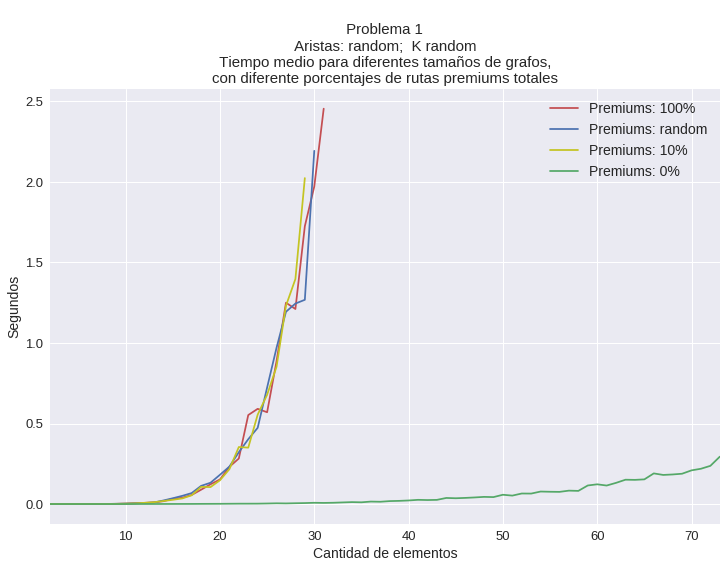
\includegraphics[width=0.9\textwidth]{imagenes/problema1/todo_random.png} \\
}

{\centering
  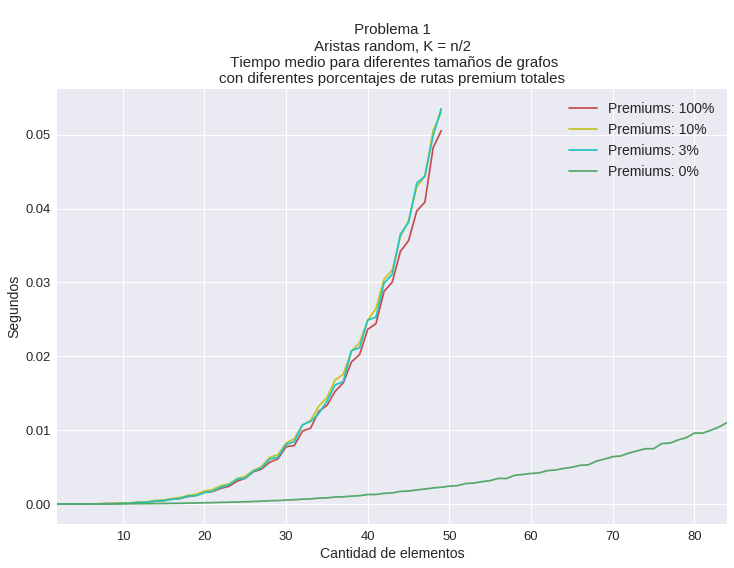
\includegraphics[width=0.9\textwidth]{imagenes/problema1/kfijo.png} \\
}

{\centering
  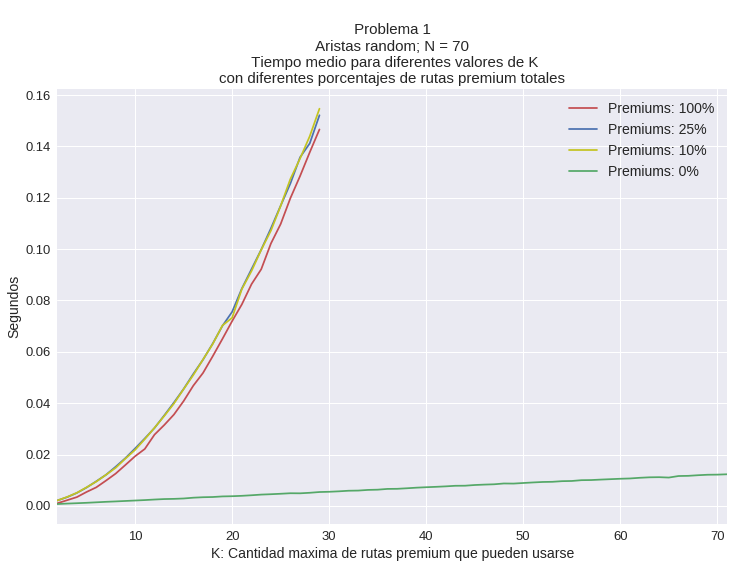
\includegraphics[width=0.9\textwidth]{imagenes/problema1/nfijo.png} \\
}

\newpage
% !TEX root = ./informe.tex

\section{Problema 2}

\subsection{Explicación}

El contexto del problema es el siguiente: tenemos un conjunto de ciudades conectadas por rutas con peajes. El costo de un peaje es cuanto se debe pagar por transitar la ruta, y el mismo puede ser negativo (uno en vez de pagar por pasar, cobra). Decimos que hay un `abuso' si podemos partir de una ciudad $c$ arbitraria y volver, teniendo un saldo positivo de dinero. El problema es encontrar el máximo $c$ que le puedo restar a todos los peajes sin que haya ningún abuso. \\

Notemos que podemos considerar a las ciudades como nodos, a las rutas como aristas, y a los peajes como el peso de las mismas; modelando el contexto como un grafo \todo{rotulado?}. Visto esto, el problema se reduce a encontrar el máximo $k$ tal que en el grafo en el que todos los pesos decrementan en $k$, no hay circuito simples negativos. \\

\subsection{Correctitud}

Supongamos que queremos calcular el camino mínimo de un nodo $a$ a $b$, en un grafo $G$ arbitrario. De haber un ciclo negativo entre ambos nodos, el algoritmo de Bellman Ford es capaz de detectarlo. Parece una buena herramienta para darnos cuenta si estamos frente a un abuso o no, pero no es tan sencillo. La sutileza consiste en notar que la ausencia de ciclos negativos entre $a$ y $b$ no implica que no exista ninguno en todo $G$. Esto puede ocurrir porque no se nos garantiza que la entrada forme un grafo orientado fuertemente conexo. Como consecuencia, podríamos llegar a tener un ciclo negativo cuyos nodos no sean alcanzables por $a$, con lo cual Bellman Ford no nos alcanzaría para detectar infaliblemente cuando no hay abuso.\\

Puede solventarse esta situación con la siguiente idea. Supongamos que tuviesemos un nodo $a$ con un camino hacia todos los nodos de nuestro grafo. De existir un ciclo negativo, todos sus nodos serían alcanzables por $a$, por lo que el mismo sería detectable aplicando Bellman Ford. Asimismo, de no existir ningún ciclo negativo, el algoritmo devolvería el mínimo recorrido hacia todos los nodos partiendo de $a$, lo cual nos informaría que no hay ciclos negativos. \\

Para aprovechar esto, dado un grafo \todo{rotulado?} $G$ válido en nuestro problema, podemos extender $G$ agregándole un nuevo nodo $u$ que tenga un arco de ida hacia todos los demás ejes. Llamemoslé a este nuevo grafo $G'$. Como acabamos de ver, aplicar Bellman Ford sobre $u$ en $G'$ nos permite determinar univocamente si hay algún circuito negativo o no. Lo que faltaría ver es que no agregamos circuitos negativos al realizar la extensión. Esto no ocurre, porque si tengo circuitos nuevos, deberán pasar por los ejes que acabamos de agregar, lo cual es absurdo, pues por construcción no hay ningún camino orientado a $u$. Entonces, los circuitos $G$ y $G'$ siguen siendo los mismos. Entonces, si aplicamos Bellman Ford desde $u$ en $G'$, podemos saber si hay ciclos negativos en $G$, o en otras palabras, si hay abuso. \\

En \texttt{EXTENDERGRAFO} lo que hacemos es conseguir la extensión. Como al crear el grafo dejamos el primer nodo `libre', lo que hacemos es usarlo como nuestro $u$. Agregamos a la lista de adyacencia de $u$ a todos los nodos que representan ciudades, y les ponemos un costo arbitrario a los nuevos ejes (en particular $0$). Al aplicarse esta función, el algoritmo de Bellman Ford va a aplicarse sobre este nuevo grafo, que como ya vimos, nos da la información que queremos sobre la entrada original. \\

La función que se encarga de implementar el algoritmo es \texttt{HAYABUSO}. Lo que hacemos en le mismo es aplicar el algoritmo de Ford $n+1$ veces, donde la última iteración se encuentra dentro de \texttt{HAYCICLONEGATIVO}, que se encarga de preguntar si las distancias mínimas de los nodos siguen cambiando. Notar que el peso que consideramos para cada eje es el peso original menos $resta$. De esta forma, estamos trabajando sobre el grafo con los pesos decrementados en $resta$, a pesar de que no lo tengamos almacenado explicitamente. Entonces, \texttt{HAYABUSO} nos devuelve si hay un ciclo negativo en el grafo restado, desde el nodo $0$ hacia todos los demás nodos. Por todo lo que vimos anteriormente, esto es lo mismo que devolver si en nuestro grafo con los pesos restados hay abuso. \\

Visto esto, analicemos el pseudocódigo de \texttt{RESOLVER} para garantizar que devuelve la respuesta correcta. En principio, observemos que consta de una búsqueda binaria sobre el rango $[0..c+2)$, donde $c$ es el máximo costo de peaje. Supongamos por un segundo que sabemos que el $k$ que buscamos está en ese rango. En cada partición de nuestro espacio de búsqueda, tomamos la mitad superior incluyendo al pivote $m$ si no hay abuso, y la mitad inferior si lo hay. Si restando $m$ tenemos un abuso, entonces sé que nuestro $k$ no es $m$ (pues estamos buscando un $k$ en el que no se produzca abuso); y que si ya con $m$ tenemos un abuso, con valores mayores lo seguiremos teniendo, por lo que puedo descartar a $m$ y la mitad superior de nuestro espacio de búsqueda. Si por el contrario, restando $m$ no nos da un abuso, entonces $m$ es un posible candidato a $k$. Los valores menores a $m$ tampoco nos darán abuso, pero son todos valores menores a $k$, y lo que estoy buscando es el máximo. Por ende, puedo descartar la mitad inferior de nuestro espacio de búsqueda. Entonces, lo que estamos buscando efectivamente es el máximo $k$ tal que no hay abuso en el grafo producto de haber decrementado todos los pesos de los ejes en $k$. \\

Ahora, ¿cómo sabemos que se encuentra el $k$ en el rango $[0..c+2)$? Bueno, no puede ser negativo, porque sabemos que sin ninguna modificación no tenemos ningún abuso. Restarle a los costos un número negativo implicaría hacer los peajes más caros, lo que haría menos posible un abuso. Tampoco puede ser mayor a $c+1$, porque como $c$ es máximo, y quedarían todos los costos de los peajes negativos. Por el enunciado, sabemos que todas las ciudades tienen una ruta de salida, con lo cual siempre podemos asegurar que tenemos un ciclo. Si todos los peajes son negativos, esto implica que tendríamos tener algún ciclo negativo. Entonces, el $k$ que buscamos está entre $0$ y $c+1$ inclusive.

\todo[inline]{En muchos lados se menciona la obviedad de que con $k$ más grande hay 'más' abuso, pero nunca se da una pseudo-demostración de por qué. Quizás no hace falta, tho.}

\newpage
\subsection{Pseudocódigo}
\todo[inline]{Falta agregar comentarios sobre las complejidades}

Vamos a utilizar como entrada en nuestro algoritmo a las siguientes variables:
\begin{itemize}
	\item $n$: La cantidad de ciudades
	\item $grafo$: El grafo de entrada representado con listas de adyacencia. Las posiciones del $1$ a $n$ representan nuestras ciudades, mientras que la posición $0$ se deja libre para la extensión
	\item $costo$: La matriz con los costos de peaje, en donde en la posición $(i,j)$ está el costo de la ruta que va desde $i$ hasta $j$
	\item $c$: El máximo costo de peaje
\end{itemize}

\begin{algorithm}
\label{resolver}         % and a label for \ref{} commands later in the document
\begin{algorithmic}
\Function{resolver}{}
	\State \Call{extenderGrafo}{()}
    \State $d \gets 0$
	\State $h \gets c + 2$
	\While{$h - d > 1$}
		\State $m \gets (h + d)/2$
		\If{$\neg$\Call{hayAbuso}{$m$}}
			\State $d \gets m$
		\Else
			\State $h \gets m$
		\EndIf
	\EndWhile
	\Return $d$
\EndFunction
\end{algorithmic}
\end{algorithm}

\begin{algorithm}
\begin{algorithmic}
\Function{extenderGrafo}{}
	\For{$i \in [1..n)$}
		\State \Call{agregarAdelante}{$grafo[0], i$}
		\State $costo[0][i] \gets 0$
	\EndFor
\EndFunction
\end{algorithmic}
\end{algorithm}

\begin{algorithm}
\begin{algorithmic}
\Function{hayAbuso}{$resta: Int$}
	\State $dist \gets$ \Call{initMatrizInfinito}{$n + 1$}
	\State $dist[0] \gets 0$
	\For{$i \in [1..n)$}
		\For{$nodo \in [0..n]$}
			\For{$vecino \in grafo[nodo]$}
				\State $peso \gets grafo[nodo][vecino] - resta$
				\State $dist[vecino] \gets$ \Call{$min$}{$dist[vecino], dist[nodo] + peso$}
			\EndFor
		\EndFor
	\EndFor
	\Return \Call{hayCicloNegativo}{$dist, resta$}
\EndFunction
\end{algorithmic}
\end{algorithm}

\begin{algorithm}
\begin{algorithmic}
\Function{hayCicloNegativo}{$dist: Int[], resta: Int$}
	\For{$nodo \in [0..n]$}
		\For{$vecino \in grafo[nodo]$}
			\State $peso \gets grafo[nodo][vecino] - resta$
			\If{$dist[vecino] > dist[nodo] + peso$}
				\Return $true$
			\EndIf
		\EndFor
	\EndFor
	\Return $false$
\EndFunction
\end{algorithmic}
\end{algorithm}

\newpage

\subsection{Complejidad}

\subsection{Experimentos}

\newpage
\section{Problema 3}
\subsection{Explicación}

--> contar el enunciado del problema

\subsection{Correctitud}

Que haya una y solo una ruta para llegar de una ciudad a cualquier otra, significa que tenemos que lograr que las rutas formen un arbol. (minimizando costo total). Construir alguna ruta o destruir alguna ruta tiene un costo asociado. Quedarme con una ruta que ya existe me cuesta 0, porque no la construyo ni destruyo. Por lo tanto, lo mas eficiente es quedarme con rutas que ya existen. \\

¿Da igual quedarme cualquier ruta ya existente? No, porque como quiero usar la minima cantidad de rutas, es posible que necesite destruir turas que estan de mas, en ese caso voy a elegir destruir las que son mas baratas de destruir. En otras palabras, priorizo quedarme con las que son mas caras de destruir. \\

Entonces, a las rutas que ya existen les asigno el \textbf{negativo} costo de destruirlas, de esta forma la ruta con el nuevo costo minimo sera en realidad la ruta con mayor costo de destrucción. En caso de necesitar rutas extra, no queda otra alternativa que construir nuevas rutas con el costo de construccion dado. \\

La solución del problema es la siguiente:
Considero el grafo \textbf{completo}. Las rutas que ya existían las coloco con su peso de destrucción negativo, y las que no existían las coloco con su peso de construcción normal. \\

Consiguiendo el arbol generador minimo, el costo total es el costo de destruccion de \textbf{todas las aristas que existían}, sumado a los costos (incluyendo negativos) de las aristas del arbol. Si la ruta del arbol era negativa, entonces se resta al costo total (esta bien pues ya existia), y si era positiva se suma al costo total (esta bien porque no existia) \\


\subsection{Pseudocódigo}


\subsection{Complejidad}

$$O(n^2)$$ usando Prim naive


\subsection{Experimentos}

ideas:\\
0 rutas existentes\\
m rutas existentes\\
random rutas existentes\\

En general todo deberia dar los mismos tiempos, porque siempre construyo el arbol completo y aplico prim al completo

\end{document}
